\documentclass[oneside,14pt]{extarticle}
\usepackage[utf8]{inputenc}
\usepackage[english,ukrainian]{babel}
\usepackage[T1]{fontenc}
\usepackage{amssymb,amsfonts,amsmath,amsthm,mathtext,textcomp}

\usepackage[includehead, headsep=0pt, footskip=0pt, top=2cm, bottom=2cm, left=2.5cm, right=1cm]{geometry}
\usepackage{indentfirst}
\usepackage[onehalfspacing]{setspace}
\usepackage[headings]{fancyhdr}
\usepackage{etoolbox}
\usepackage{flafter}
\usepackage{listings}
\usepackage{graphicx}
\usepackage{float}
\usepackage[center]{titlesec}
\PassOptionsToPackage{hyphens}{url}\usepackage{hyperref}
\usepackage{array}
\fancyhf{}
\renewcommand{\headrulewidth}{0pt}
\fancyhead[R]{\thepage}
\pagestyle{fancy}
\fancypagestyle{plain}{%
	\fancyhf{}
	\fancyhead{}
	\fancyfoot{}
	\fancyhead[RO]{\thepage}
	\fancyhead[LE]{\thepage}
	\renewcommand{\headrulewidth}{0pt}
	\renewcommand{\footrulewidth}{0pt}
}
\lstset{breaklines=true,showstringspaces=false}
\graphicspath{ {./pictures} }
\counterwithin{figure}{section}
\titlelabel{\thetitle.\quad}
\renewcommand*{\thesection}{Розділ~\arabic{section}}
\renewcommand*{\thesubsection}{\arabic{subsection}}
\renewcommand{\thefigure}{\arabic{section}.\arabic{figure}}
\usepackage{tocloft}
\setlength{\cftsecnumwidth}{5em}
\setlength\parindent{1.25cm}
\usepackage{enumitem}

\begin{document}
\begin{titlepage}
	\begin{center}
		Національний університет <<Львівська політехніка>>\\
		Кафедра програмного забезпечення
		
		\vspace{40pt}
		\textbf{\LARGE КУРСОВА РОБОТА}\\
		{\large
		\textbf{з дисципліни <<Бази даних>>}\\
		на тему:\\
		<<Інформаційна система для компанії з регулярних перевезень>>
		}
		\vspace*{40pt}
		
		\begin{flushright}
		    \begin{minipage}{0.6\textwidth}
		        \underline{Виконав}:\\
                Стедент спеціальності 121\\
			    <<Інженерія програмного забезпечення>>\\
			    групи ПЗ-32\\
			    Коваленко Д.М.
			    \bigbreak
			    
			    \underline{Керівник}:\\
			    асистент кафедри програмного забезпечення\\
			    Білоіваненко М.В.
			    \bigbreak
			    
			    \underline{Оцінка}:\\
			    Національна шкала \rule{6.35cm}{0.15mm}\\			
			    Кількість балів \rule{2cm}{0.15mm} Оцінка ECTS \rule{2cm}{0.15mm}
			    \bigbreak
            \end{minipage}
		\end{flushright}
		\vspace{40pt}
		Члени комісії \hspace{1.9cm} \rule{3cm}{0.15mm} \hspace{1cm} Білоіваненко М.В.\\
		{\small\vspace{-5pt}(підпис)}\\
		\hspace{2.65cm}\hspace{1.9cm}  \rule{3cm}{0.15mm} \hspace{1cm} Цимбалюк Т.М.\\
		{\small\vspace{-5pt}(підпис)}\\
		
		\vspace{\fill}
		Львів — 2024
	\end{center}
\end{titlepage}
\setcounter{page}{2}
\tableofcontents
\newpage

\section{Аналіз предметної області та постановка завдання}
\subsection{Опис предметної області}
Інформаційна система для компанії з регулярних перевезень створюється для оптимізації управління пасажирськими перевезеннями шляхом автоматизації процесів призначення водіїв, ведення обліку пасажирів та квитків, а також аналізу.

Інформаційна система для компанії з регулярних перевезень також надає можливість пасажирам отримувати доступ до розкладу руху транспортних засобів та іншої корисної інформації. Пасажири можуть скористатися додатком для перегляду актуального розкладу руху автобусів, зупинок та часу їх прибуття на кожну зупинку.

% Актуальність
З кожним днем мобільність населення постійно зростає, транспортна інфраструктура розвивається, потреба у вдосконаленні та оптимізації процесів управління перевезеннями постійно росте. Компанії, які здійснюють регулярні перевезення, стикаються з великою кількістю даних, складних розрахунків і потребують ефективних інструментів для керування цими процесами. Розробка інформаційної системи для компанії з регулярних перевезень стає необхідністю для оптимізації витрат, підвищення якості обслуговування та конкурентоспроможності.

% Специфікація важливих понять
\begin{list}{-}{Специфікація важливих понять:}
\item Зупинка - інформація про місце, призначене для посадки та висадки пасажирів.
\item Маршрут - послідовність зупинок, які обслуговує певний транспортний засіб.
\item Транспортний засіб - засіб перевезення пасажирів, який обслуговує певний маршрут.
\item Водій - особа, яка керує транспортним засобом під час перевезення пасажирів.
\item Квиток - інформація про проїзну карту видану пасажиру.
\item Транзакція - запис, що фіксує факт використання квитка пасажиром на конкретному маршруті та у певний час.
\item Розклад руху - перелік часу прибуття та відправлення транспортного засобу на кожній зупинці певного маршруту.
\item Технічне обслуговування транспортних засобів - заправка, зміна шин, загальний огляд, прибирання, тощо.
\end{list}

% Встановлення обсягів аналізу теми
Аналіз предметної області буде обмежений на даних про перевезення пасажирів автобусами, не включаючи трамваї, метро, залізничний транспорт, пароми, канатні дороги, гондоли, фунікулери, тощо.

\subsection{Вимоги до обробки даних}
% Опис актуальних бізнес процесів
Бізнес-процеси компанії з регулярних перевезень пасажирів включають ряд дій та етапів, які забезпечують ефективну організацію та функціонування пасажирських перевезень. Компанія визначає регулярні маршрути, графіки руху та зупинки для пасажирських транспортних засобів. Це включає вибір оптимальних маршрутів, розподіл транспортних засобів та встановлення годин руху. Призначення водіїв на кожен транспортний засіб.

% Опис накопичення та аналізу даних
Для ефективного управління пасажирськими перевезеннями необхідно накопичувати та аналізувати різноманітні дані. Зокрема збір інформації про рух транспортних засобів, кількість пасажирів на кожній зупинці, реєстрацію квитків та транзакцій, а також звіти про витрати і доходи. Аналіз цих даних допоможе виявити шаблони в руху пасажирів, визначити популярні маршрути та години, забезпечити достатню кількість транспортних засобів для попиту, а також виявити ефективність роботи водіїв та рейсів.

% Деталізація інформаційних структур
База даних для інформаційної системи компації з регулярних перевезень повинна містити наступні ключові сутності:
\begin{itemize}
\item Зупинка - інформація про місце, призначене для посадки та висадки пасажирів.
\item Маршрут - послідовність зупинок, які обслуговує певний транспортний засіб.
\item Транспортний засіб - засіб перевезення пасажирів, який обслуговує певний маршрут.
\item Водій - особа, яка керує транспортним засобом під час перевезення пасажирів.
\item Квиток - інформація про проїзну карту видану пасажиру.
\item Транзакція - запис, що фіксує факт використання квитка пасажиром на конкретному маршруті та у певний час.
\item Розклад руху - перелік часу прибуття та відправлення транспортного засобу на кожній зупинці певного маршруту.
\end{itemize}

\subsection{Постановка завдання}
% Перелік необхідних функцій інформаційної системи
Інформаційна система для компанії з регулярних перевезень повинна мати ряд ключових функцій, що забезпечують ефективне управління та оптимізацію бізнес-процесів. Перш за все, система повинна забезпечувати зберігання та оновлення інформації про перевезення пасажирів, доступні маршрути та транспортні засоби.

З урахуванням періодичної природи бізнесу, система має підтримувати пов’язані з часом події, такі як регулярні рейси, їх час та тривалість, а також фіксувати дані про пасажирів і операції щодо їх перевезення. Вона також повинна забезпечувати можливість аналізу цих даних для виявлення тенденцій та оптимізації ресурсів.

\begin{list}{•}{Інформаційна система для компанії з регулярних перевезень повинна мати наступні функції:}
    \item Довготривале зберігання та оновлення даних про перевезення пасажирів, транспортні засоби та маршрути.
    \item Можливість внесення нових даних та редагування існуючих з урахуванням обмежень цілісності.
    \item Функції сортування, вибірки та пошуку інформації для аналізу та оптимізації бізнес-процесів.
    \item Представлення даних у зручній табличній формі для зручного аналізу та використання.
    \item Інтерактивний інтерфейс користувача, що відповідає логіці бізнес-процесів компанії.
\end{list}
\newpage

\section{Розробка моделей зберігання даних}
\subsection{Концептуальне проектування}
% Взаємозв’язки та характеристики понять, що описані в базі даних
Основними структурами інформаційної системи для компанії з регулярних перевезень визначено наступні компоненти:
\begin{itemize}
\item Зупинка
\item Маршрут
\item Розклад
\item Транспортний засіб
\item Водій
\item Квиток
\item Транзакція
\item Технічне обслуговування
\item Види пільг для квитка
\end{itemize}

Основними зв'язками між переліченими сутностями можна визначити наступні відношення:
\begin{itemize}
\item Маршрут - зупинка (many to many): маршрут може містити кілька зупинок, кожна зупинка може належати кільком маршрутам.
\item Квиток - транзакція (one to many): кожен квиток може бути пов'язаний з багатьма транзакціями, транзакція може мати лише один асоційований квиток.
\item Водій - транспортний засіб (one to one): кожен водій може бути пов'язаний лише з одним транспортним засобом.
\item Транспортний засіб - маршрут (one to one): кожен транспортний засіб може бути пов'язаний лише з одним маршрутом.
\end{itemize}

\subsection{Вимоги до системи накопичення даних}
% Оцінка обсягів даних
Обсяги даних, що будуть зберігатися в інформаційній системі для компанії з регулярних перевезень, залежать в першу чергу від масштабів та рівня розвитку мережі транспортного сполучення. Беручи до уваги розмір первинних історичних даних для міста Мельбурн (Австралія), можна припустити, що база даних буде містити в середньому кілька сотень маршрутів, кілька тисяч зупинок та близько мільйона записів про розклад руху, при цьому необхідно зберігати інформацію про тисячу транспортних засобів та водіїв, а також обробляти близько трьох мільйонів транзакцій від двох мільйонів пасажирів щодня.

% Частота додавання
Очевидно найзатребуванішими ресурсами бази даних для додавання, буде інформація про транзакції та пасажирів. Іншим затребуваним ресурсом для додавання може бути інформація про обслуговування транспортних засобів, особливо під час початку або завершення робочого дня, коли проводиться технічне обслуговування транспортних засобів.

Для читання найзатребуванішими запитами буде отримування розкладу руху для пасажирів та деталей маршруту для водія.

% Очікувані запити та вибірки
Очікувані запити та вибірки для інформаційної системи для компанії з регулярних перевезень можуть включати:
\begin{itemize}
\item Отримання розкладу руху: Користувачі, особливо пасажири, можуть бажати отримати інформацію про час прибуття та відправлення транспортного засобу на конкретній зупинці або для певного маршруту.
\item Пошук маршрутів за двома зупинками: Користувачі можуть шукати маршрути між двома певними зупинками, щоб планувати свої поїздки.
\item Пошук зупинок за назвою: Користувачі можуть шукати зупинки за їхніми назвами або частковими співпадіннями.
\item Отримання інформації про обслуговування транспортного засобу: Адміністратори або водії можуть бажати отримати інформацію про проведене технічне обслуговування транспортного засобу, включаючи опис робіт, вартість та дату проведення обслуговування.
\end{itemize}

% Обмеження доступу та ін.
Для обмеження доступу користувачів було створено три основні ролі - \textit{passenger}, \textit{driver}, \textit{manager}.

\begin{itemize}
\item \textit{passenger} - має доступ до отримання розкладу руху на вказаній зупинці, та можливість пошуку маршрутів між двома зупинками. Такод має право створювати транзакції.
\item \textit{driver} - може додавати дані до таблиці \textit{maintenance}, та отримувати дані про поточний маршрут.
\item \textit{manager} - має повний доступ до всіх даних.
\end{itemize}

\subsection{Логічне проектування схеми бази даних}
% Домени
Основними доменами схеми бази даних передбачено дані для пасажирів (розклад руху, квитки, транзакції), дані для водіїв (розклад руху, записи про технічне обслуговування транспортних засобів) та менеджерів (управління розкладом руху, маршрутами, тощо).

% Таблиці
База даних для предметної області складається з наступних структур:
\begin{itemize}
\item Таблиця \textit{Stop} містить дані про назву та розміщення (широта, довгота) місць, де транспорт зупиняється для посадки та висадки пасажирів.
\item Таблиця \textit{Route} містить дані про коротку та повну назву маршрутів руху транспорту.
\item Таблиця \textit{Driver} містить дані про ім'я водія та ідентифікаційний номер транспортного засобу, що призначений водієві.
\item Таблиця \textit{Vehicle} містить дані про номерний знак транспортого засобу та кількість місць для пасажирів.
\item Таблиця \textit{Maintenance} містить дані про ідентифікаційний номер транспортного засобу та водія, опис, вартість та час проведення обслуговування.
\item Перелічуваний тип \textit{Ticket\_discount} вказує на вид пільги квитка, містить варіанти \textit{student}, \textit{elder}, \textit{veteran}.
\item Таблиця \textit{Ticket} містить дані про тип пільги, якщо така існує, та доступний баланс.
\item Таблиця \textit{Transaction} містить дані про ідентифікаційний номер квитка, маршруту, транспортного засобу, зупинки на якій відбулась посадка пасажира, зупинка на якій відбулась висадка пасажира, вартість проїзду  та час.
\item Таблиця \textit{Schedule} містить дані про ідентифікаційний номер маршруту, зупинки, та час прибуття і відправлення.
\item Таблиця \textit{Route\_stops} містить дані про ідентифікаційний номер маршруту, зупинки та порядковий номер зупинки на маршруті.
\item Таблиця \textit{Route\_vehicles} містить дані про ідентифікаційний номер маршрутів та транспортних засобів.
\end{itemize}

\subsection{Реалізація процедур бізнес-логіки}
% Тригери
Для реалізації бізнес-логіки не було використано тригери.

% Процедури
Для реалізації бізнес-логіки реалізовано наступні процедури:
\begin{itemize}
\item \textit{new\_transaction} - інкапсулює логіку створення нової транзакції. Виконує валідацію вхідних даних відповідно до обмежень цілісності бази даних, виконує списання коштів з рахунку квитка, та створює новий запис у таблиці транзакцій.
{\fontsize{8pt}{8pt}\selectfont\begin{lstlisting}[language=sql]
create or replace function new_transaction(ticket_id uuid, vehicle_id character varying(16), from_stop_id integer, to_stop_id integer)
returns void as
$$
declare
	fare integer;
	r_id integer = (select route_id from vehicle v where v.license = vehicle_id);
	begin
	if r_id is null then return; end if;

	fare = abs((select ord_idx from route_stops rs
	where rs.route_id = r_id and rs.stop_id = to_stop_id)
	- (select ord_idx from route_stops rs
	where rs.route_id = r_id and rs.stop_id = from_stop_id)) * 5 * coalesce((select mult from ticket_discount_mult d where d.discount = (select discount from ticket t where t.id = ticket_id)), 1);
	
	if fare is null then raise 'invalid vehicle_id for given stops'; end if;
	
	if (select balance from ticket t where t.id = ticket_id) - fare < 0 then raise 'not enough balance'; end if;
	
	update ticket t set balance = balance - fare where t.id = ticket_id;

	insert into transaction(ticket_id, route_id, vehicle_id, from_stop_id, to_stop_id, fare, timestamp)
	values (ticket_id, r_id, vehicle_id, from_stop_id, to_stop_id, fare, now());
end;
$$
	language plpgsql;
\end{lstlisting}}
\end{itemize}

% Функції
Для реалізації бізнес-логіки реалізовано наступні функції:
\begin{itemize}
\item \textit{search\_stop} - повертає зупинки, назва яких частково співпадає з аргументом.
{\fontsize{8pt}{8pt}\selectfont\begin{lstlisting}[language=sql]
create or replace function search_stop(s varchar)
returns table (
	id integer,
	name varchar,
	lat numeric,
	lon numeric
)
language plpgsql
	as $$
	begin
		return query execute '
		select id, name, lat, lon from public.stop
		where name ilike \$1
		limit 10;
		' using '%' || s || '%';
end;
$$;
\end{lstlisting}}
\item \textit{search\_route} - повертає маршрути, назва яких частково співпадає з аргументом.
{\fontsize{8pt}{8pt}\selectfont\begin{lstlisting}[language=sql]
create or replace function search_route(s varchar)
returns table (
	id integer,
	route_name varchar
)
language plpgsql
as $$
	begin
	return query execute '
		select id, (case when name is null then full_name else name end) as route_name
		from public.route
		where name ilike \$1 or full_name ilike \$1
		limit 10;
		' using '%' || s || '%';
	end;
$$;
\end{lstlisting}}
\end{itemize}

% Представлення
Для реалізації бізнес-логіки реалізовано наступні представлення:
\begin{itemize}
\item \textit{routes\_with\_stops} - повертає маршрути які містять у собі дві вказані зупинки.
{\fontsize{8pt}{8pt}\selectfont\begin{lstlisting}[language=sql]
create view public.routes_with_stops as
	select
			s1.id as from_stop_id,
			s1.name as from_stop_name,
			s2.id as to_stop_id,
			s2.name as to_stop_name,
			r.id as route_id,
			(case when r.name is null then r.full_name else r.name end) as route_name
		from stop s1
		cross join stop s2
		join route_stops rs1 on rs1.stop_id = s1.id
		join route_stops rs2 on rs2.stop_id = s2.id
		join route r on rs1.route_id = rs2.route_id and rs1.route_id = r.id
		where s1.id <> s2.id;
alter view public.routes_with_stops owner to root;
\end{lstlisting}}
\item \textit{arrival\_with\_stops\_in} - повертає час, що залишається до прибуття до вказаної зупинки, та напрямок руху транспорту на вказаній зупинці.
{\fontsize{8pt}{8pt}\selectfont\begin{lstlisting}[language=sql]
create view arrival_with_stops_in as
select from_stop_id, from_stop_name, to_stop_id, to_stop_name, route_id, route_name, to_char(arr_in, 'MI:SS') as arr_in from (
select
		s.from_stop_id,
		s.from_stop_name,
		s.to_stop_id,
		s.to_stop_name,
		s.route_id,
		(case when r.name is null then r.full_name else r.name end) as route_name,
		sch.arr - now()::time as arr_in
	from routes_with_stops s
	join schedule sch on s.route_id = sch.route_id and (s.from_stop_id = sch.stop_id or s.to_stop_id = sch.stop_id)
	join route r on r.id = s.route_id) as arrival
	where arr_in > interval '0 seconds' and arr_in < interval '1 hour'
	order by arr_in;
alter view public.arrival_with_stops_in owner to root;
\end{lstlisting}}
\end{itemize}

\newpage

\section{Розробка програмного коду}
\subsection{Обґрунтування обраної архітектури}
% Тип
Для розробки інформаційної системи для компанії з регулярних перевезень було обрано клієнт-серверну архітектуру, що дозволить абстрагуватися над реалізацією інтерфейсу користувача, що буде корисно для підтримки різноманітних форматів взаємодії з користувачем. В реальних умовах це дозволить створити мобільний додаток для пасажирів, вбудовану систему для водіїв та додаток для персонального комп'ютера для менеджера.

Для реалізації серверної частину було використано архітектуру MVC, (Model-View-Controller) - дозволяє розділити логіку обробки даних, від логіки представлення та отримання даних.

% Мова програмування
Для реалізації серверної частини інформаційної системи для компанії з регулярних перевезень було обрано мову програмування \textit{Go}. Завдяки своїй простоті цей вибір дозволить швидко створити прототип системи. А завдяки швидкості виконання цей вибір дозволить зосередитись на створенні нового функціоналу системи замість оптимізації існуючого.

% Система баз даних
Для реалізації бази даних інформаційної системи для компанії з регулярних перевезень було обрано \textit{PostgreSQL}, що завдяки своїй популярності та зрілості дозволить швидко створити необхідний функціонал.

% Формати
Для передачі інформації з серверу на клієнт було використано формат даних \textit{JSON}. Цей формат забезпечує зручність у взаємодії з іншими програмами та забезпечує можливість збереження ієрархічної структури даних. Крім того, JSON є легким для розуміння і обробки як людьми, так і комп'ютерами, що робить його ідеальним вибором для передачі даних.

% Протоколи
Для забезпечення надійного обміну даними між клієнтом та сервером використовується гіпертекстовий протокол передачі даних (HTTP). Використання HTTP дозволяє забезпечити швидку та ефективну комунікацію, що є ключовим аспектом для коректної роботи інформаційної системи.

\subsection{Структурна модель інформаційної системи}
Програмна модель інформаційної системи для компанії з регулярних перевезень складається з наступних  частин:

\begin{itemize}
\item Серверна частина - містить модулі для взаємодії з базою даних, та модулі роботи з мережою.
\item Клієнтська частина - містить модулі інтерфейсу, та модулі роботи з серверною частиною.
\end{itemize}

\begin{figure}[H]
	\centering
	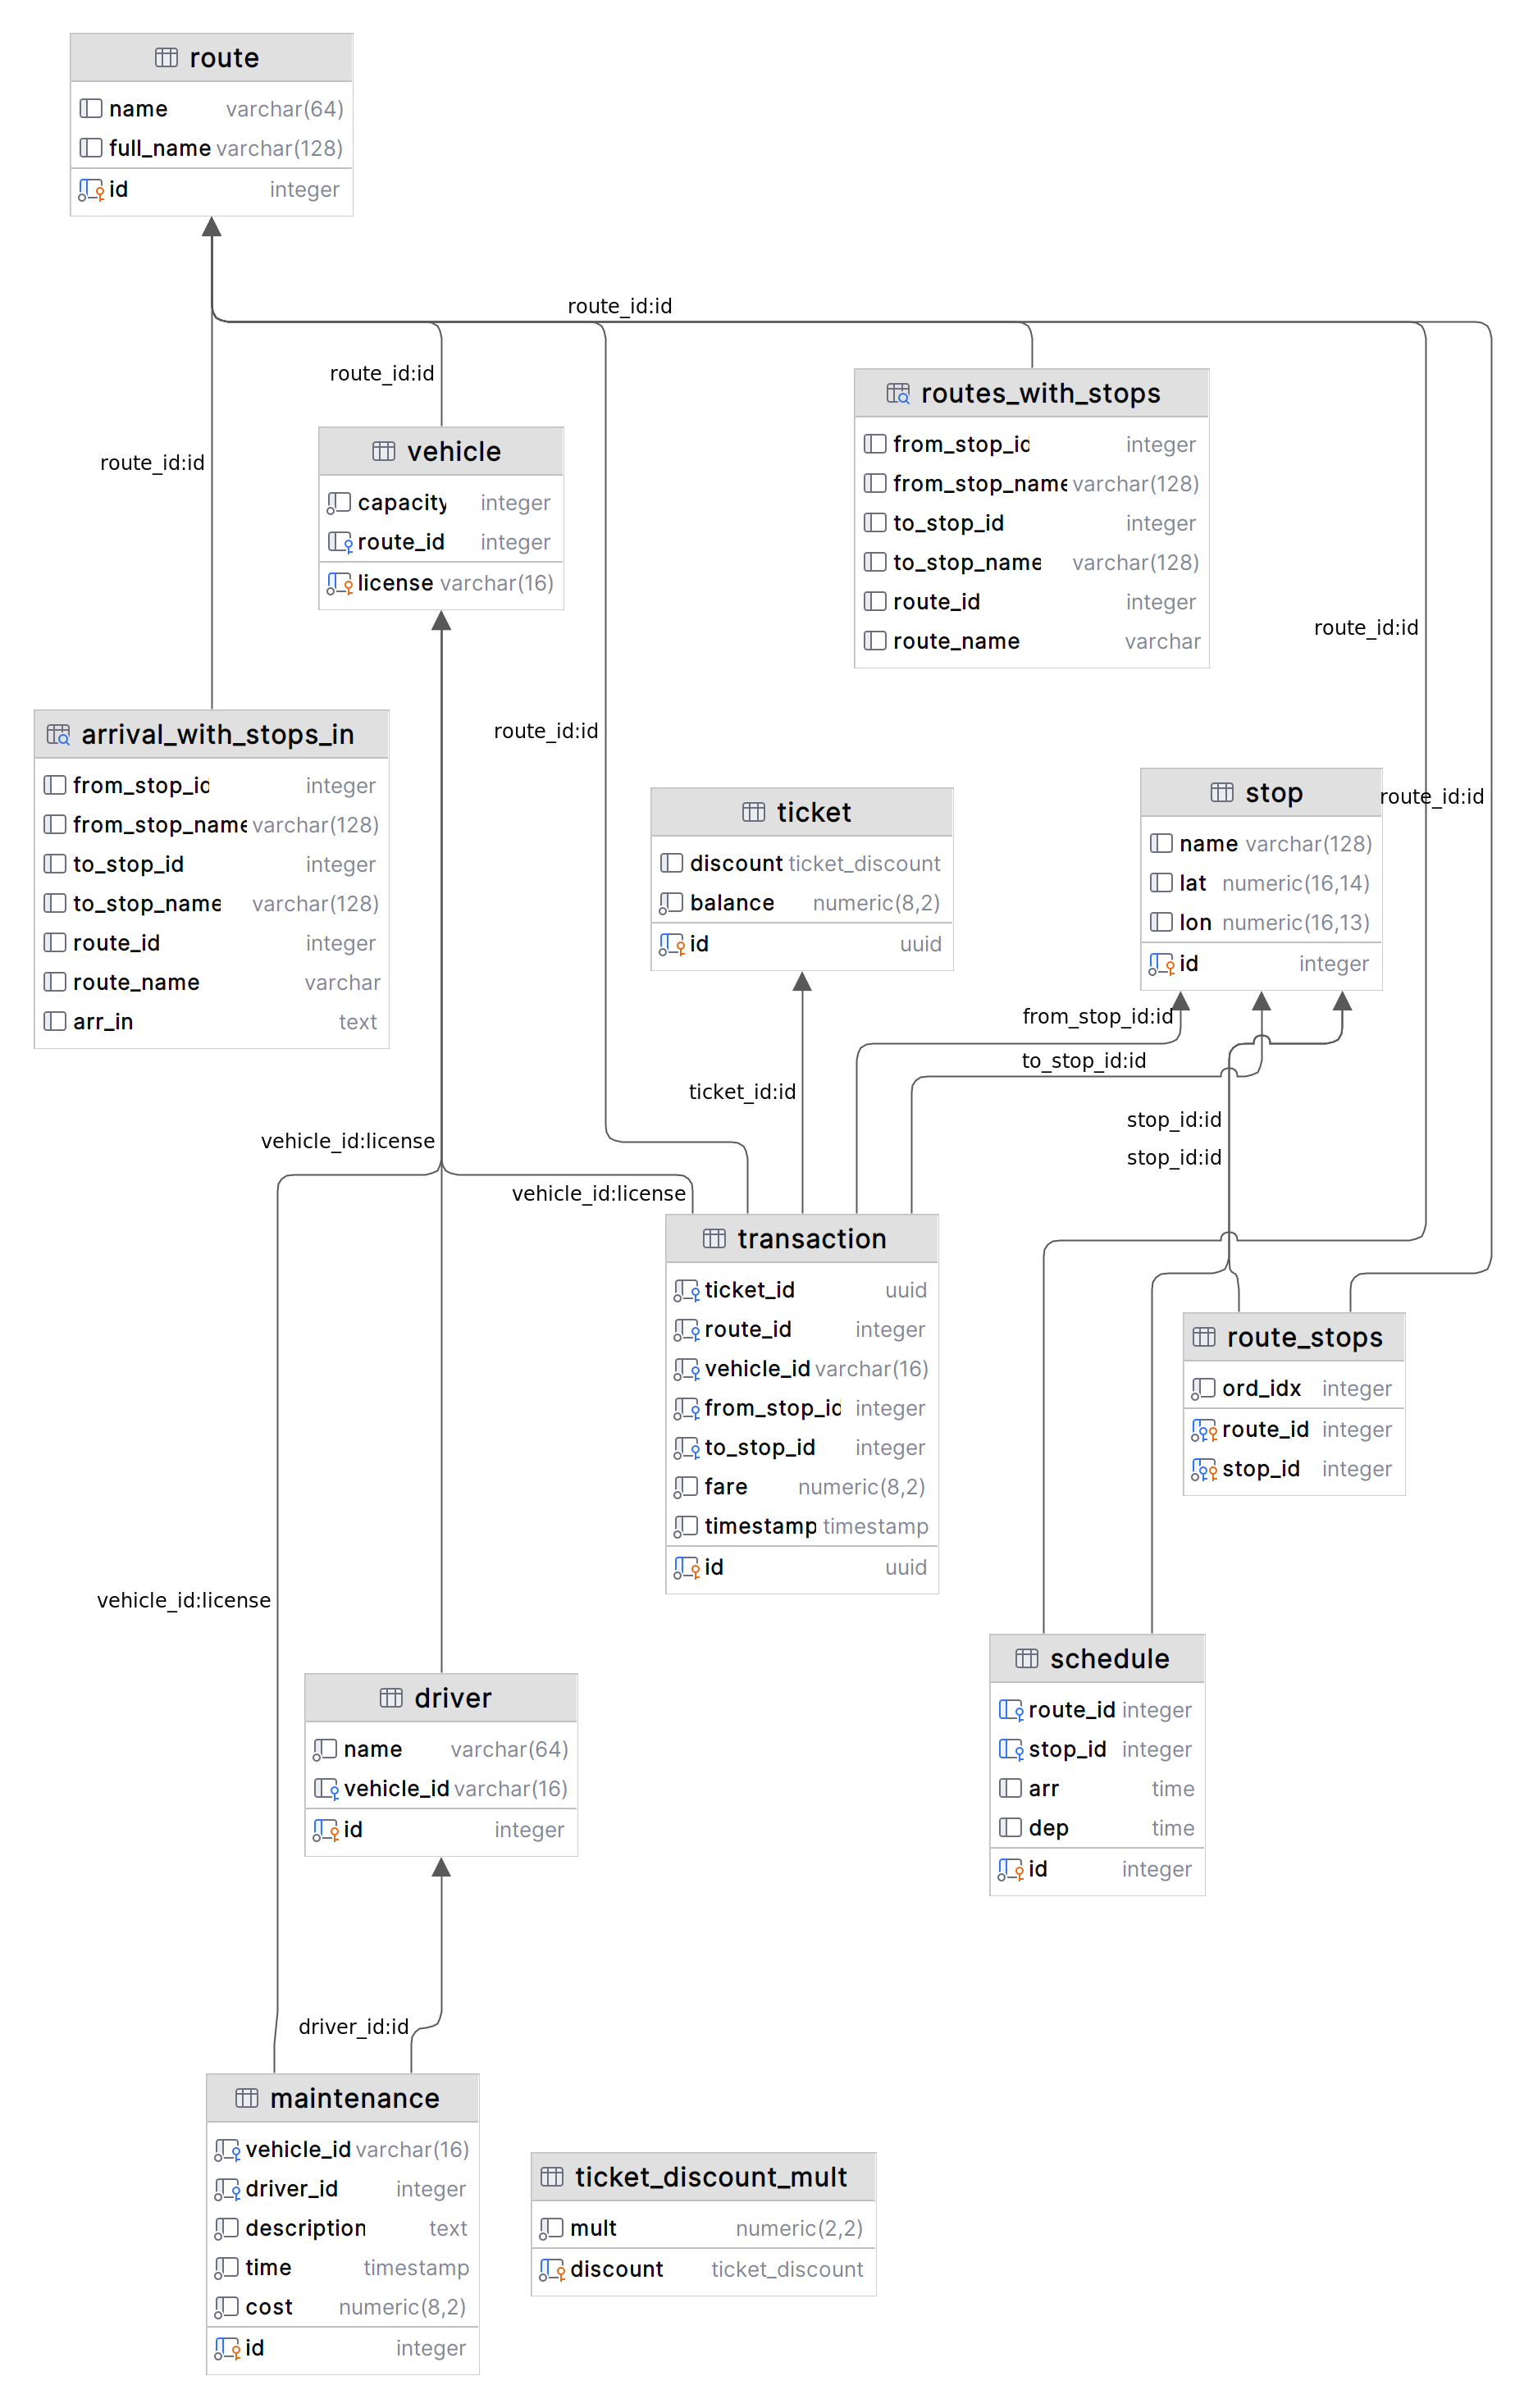
\includegraphics[scale=0.15]{schema}
	\caption{Структурна модель бази даних.}
\end{figure}

\subsection{Призначення модулів та компонентів системи}
Серверна частина містить наступні модулі:
\begin{itemize}
\item Модуль, що описує моделі бази даних, та структури даних для передачі по мережі.
\item Модуль роботи з мережею, звертається до бази даних, перетворює отриману інформацію до потрібного формату та відправляє до клієнтської частини.
\end{itemize}

Клієнтська частина має наступні модулі:
\begin{itemize}
\item Модуль для пошуку зупинок, відображає поле для пошуку, та меню для автодоповнення.
\item Модуль для пошуку маршрутів, відображає поле для пошуку, та меню для автодоповнення.
\item Модуль для відображення часу прибуття транспортних засобів до вказаної зупинки на вказаному маршруті.
\item Модуль для відображення маршрутів, що з'єднують вказані зупинки.
\item Модуль для додавання даних про технічне обслуговування транспортних засобів.
\item Модуль для експорту даних із вказаної таблиці.
\end{itemize}

\subsection{Особливості реалізації та елементи інтерфейсу}
При розробці інтерфейсу користувача було приділено особливу увагу забезпеченню простоти та зручності використання. Елементи інтерфейсу були ретельно підібрані та стилізовані з метою максимальної інтуїтивності та естетичного вигляду. Кожен модуль системи виконує свою функцію точно та ефективно, забезпечуючи високу продуктивність та надійність роботи системи в цілому.

Реалізація інтерфейсу користувача має бути реалізована наступним чином:
\begin{itemize}
	\item Якщо користувач не авторизований, він має доступ до елементів, що доступні користувачу з роллю пасажира.
	\item Користувач має можливість авторизуватися, змінивши свою роль.
	\item Якщо користувач авторизувався, то головна сторінка має змінитись відповідно до ролі користувача.
	\item Додаток має відображати отримані дані у вигляді таблиць, та має можливість їх зручно модифікувати, сортувати, фільтрувати.
	\item Додаток повинен відображати статистичні дані про прибуток.
	\item Додаток повинен мати можливість експортувати дані таблиць.
\end{itemize}

\newpage

\section{Наповнення бази даних}
\subsection{Опис джерела історичних даних}
Джерело історичних даних описує мережі громадського транспорту 25 міст по всьому світу в кількох простих у використанні форматах даних. Ці формати даних включають списки меж мережі, тимчасові списки мережевих подій, бази даних SQLite, файли GeoJSON і сумісні ZIP-файли General Transit Feed Specification (GTFS).

Вихідні дані для створення цих мереж були опубліковані агентствами громадського транспорту у форматі даних GTFS. Для створення витягів мережевих даних для кожного міста вихідні дані були відібрані на наявність помилок, відфільтровані просторово й у часі та доповнені пішохідними відстанями між зупинками громадського транспорту за допомогою даних OpenStreetMap.

Для виконання роботи були використані дані для міста Мельбурн (Австралія), що складаються з 467 маршрутів, 19649 зупинок, 2714796 записів про розклад руху.

\subsection{Опис процесів генерації тестових даних}
Тестові дані генеруються за допомогою бібліотеки Faker для Python та SQL команд з використанням функції \textit{random()}, після чого адаптуються до реляційних відношень та обмежень цілісності бази даних. 

Випадковим чином були згенеровані дані для наступних таблиць: \textit{Vehicle} (1 500 записів), \textit{Driver} (2 000 записів) \textit{Ticket} (1 000 записів), \textit{Transaction} (1 000 000 записів), \textit{Maintenance} (1 000 записів).

\subsection{Трансформація та первинне завантаження даних}
Завантаження первинних історичних даних з мережі, запуск серверу бази даних, додавання рядків після створення відповідних таблиць та відношень реалізована в контейнеризованому оточенні за допомогою \textit{podman}, що дозволяє отримати готову до роботи, заповнену інформацією базу даних на будь якій системі за лічені хвилини.

Джерело первинної інформації містить багато додаткових даних, зокрема інформація про маршрути у форматі \textit{GEOjson}, що дозволяє переглядати їх за допомогою технології OpenStreetMap. Тому для отримання необхідних даних для опису предметної області були використані різноманітні шляхи видобування інформації, зокрема: 
\begin{itemize}
\item Перенесення даних з \textit{SQLite} до \textit{PostgreSQL} за допомогою перетворення даних у формат \textit{csv} та внесення в базу даних за допомогою команди \textit{copy}.
\item Вибірка необхідних даних з існуючих таблиць та їх перетворення до необхідного формату.
\end{itemize}

\newpage

\section{Функціональні можливості для користувача}
\subsection{Опис інтерфейсу у відповідності до бізнес-процесів}
Інтерфейс користувача дозволяє авторизуватися використовуючи логін та пароль, та, залежно від ролі користувача - виконувати різні дії над даними відповідно до бізнес-процесів.

\begin{figure}[H]
\centering
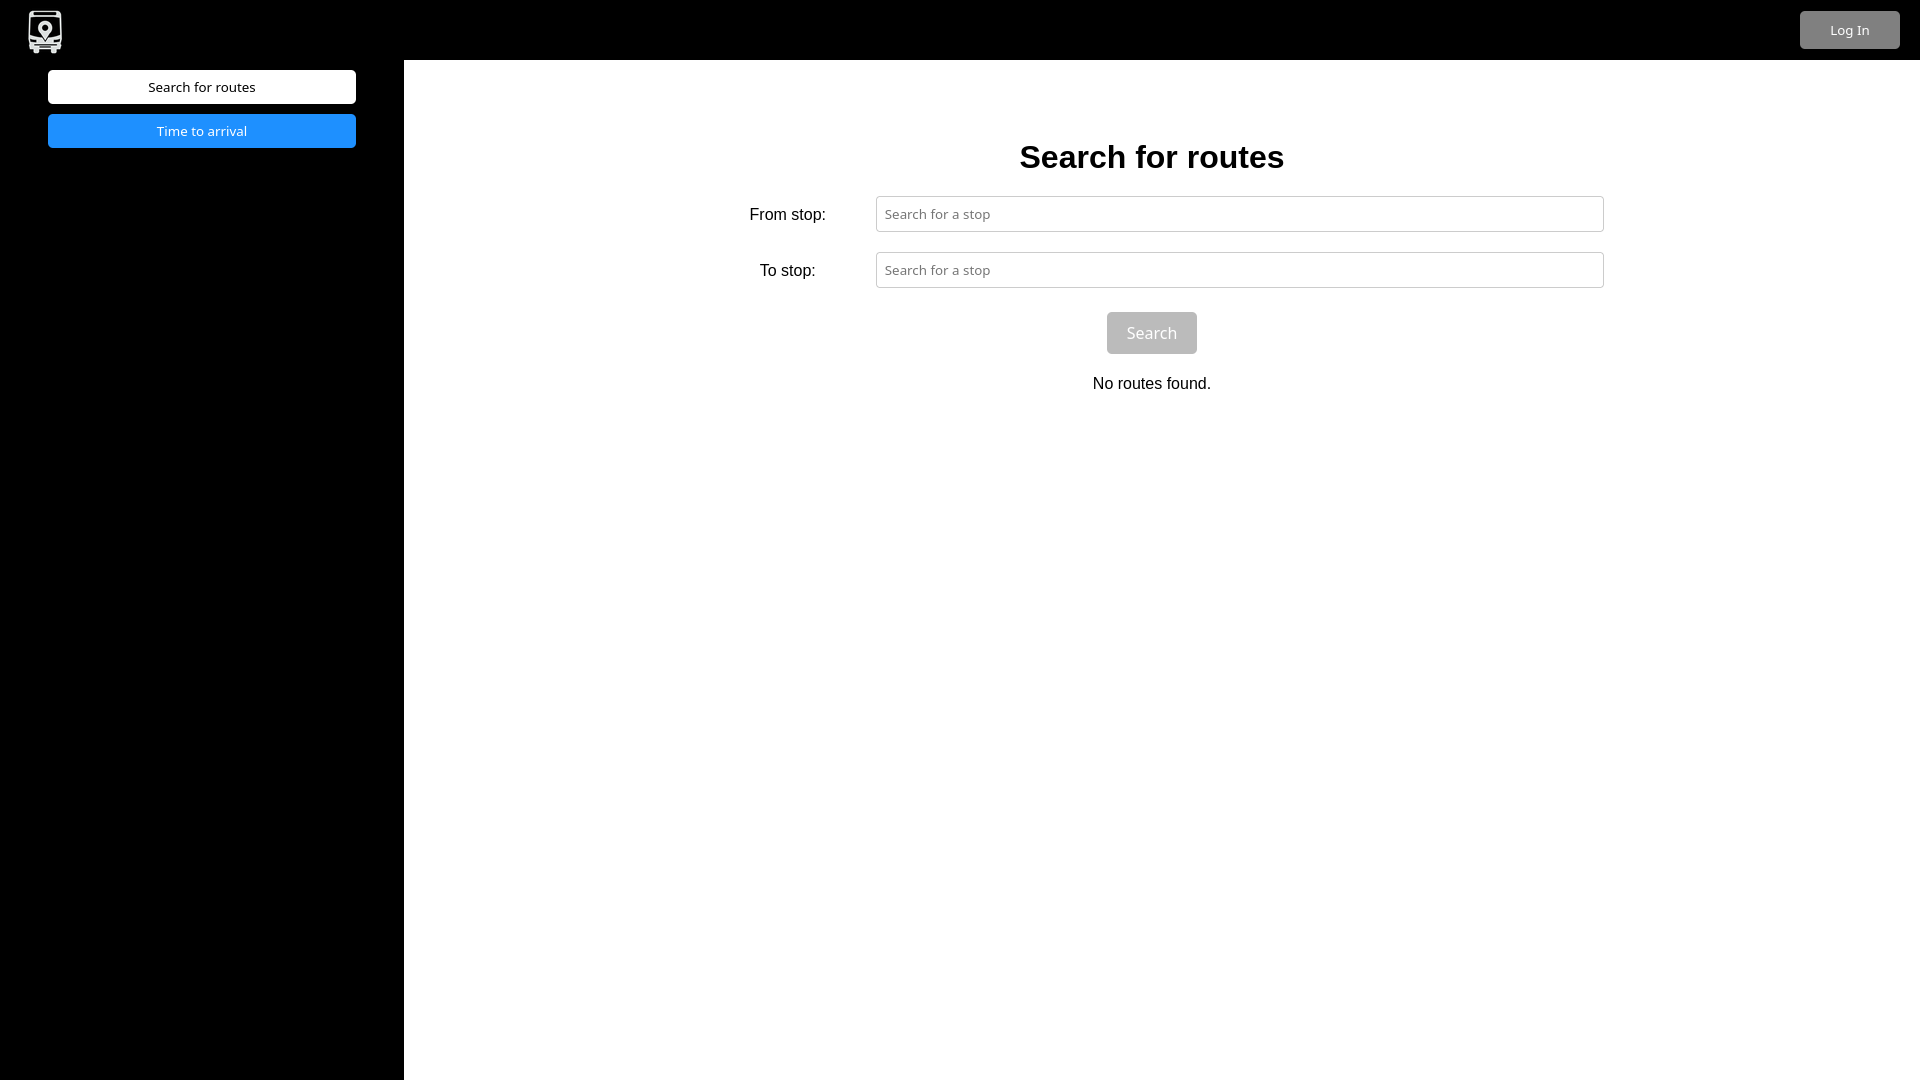
\includegraphics[scale=0.25]{1}
\caption{Сторінка пошуку маршрутів між зупинками.}
\end{figure}

Користувачі, авторизовані з роллю \textit{passenger}, мають можливість знайти маршрут між двома вказаними зупинками та отримати час до прибуття транспортного засобу на вказану зупинку на вказаному маршруті.

\begin{figure}[H]
\centering
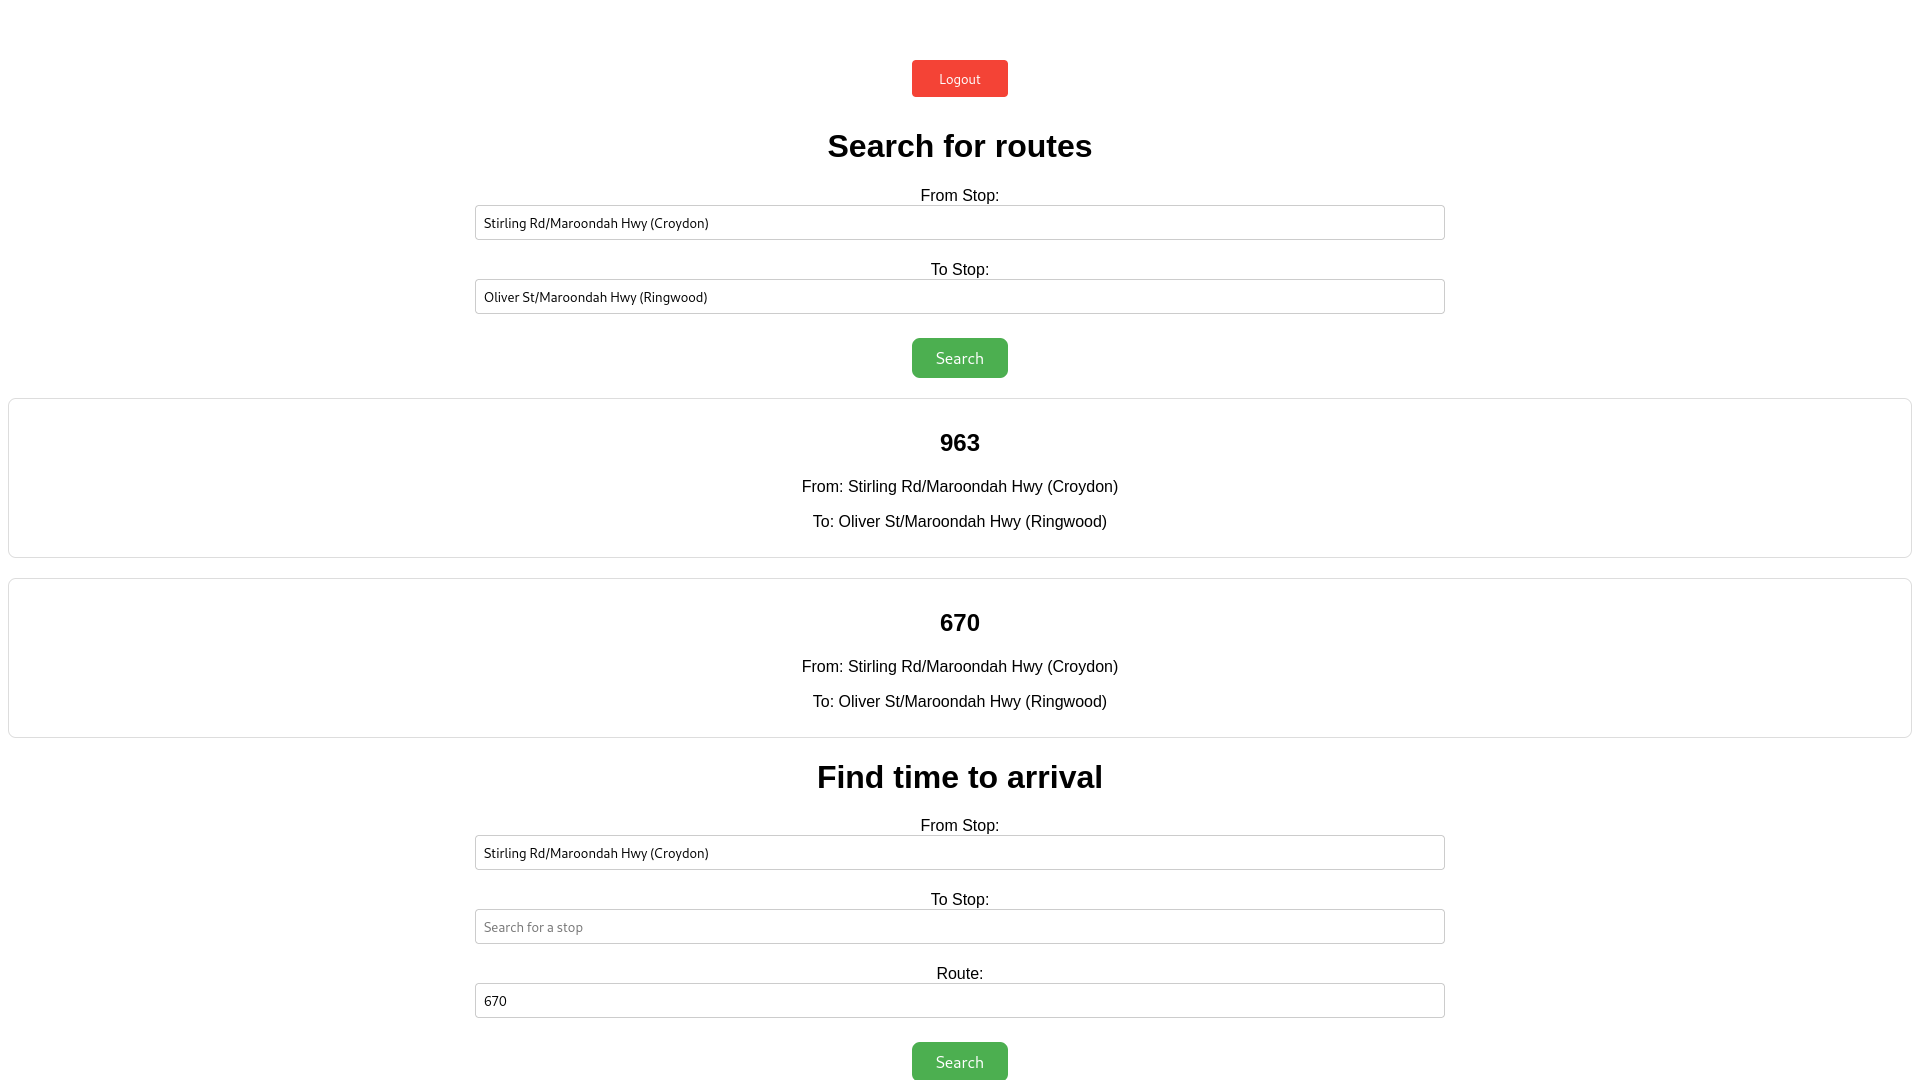
\includegraphics[scale=0.3]{2}
\caption{Сторінка пошуку маршрутів між зупинками.}
\end{figure}

\begin{figure}[H]
\centering
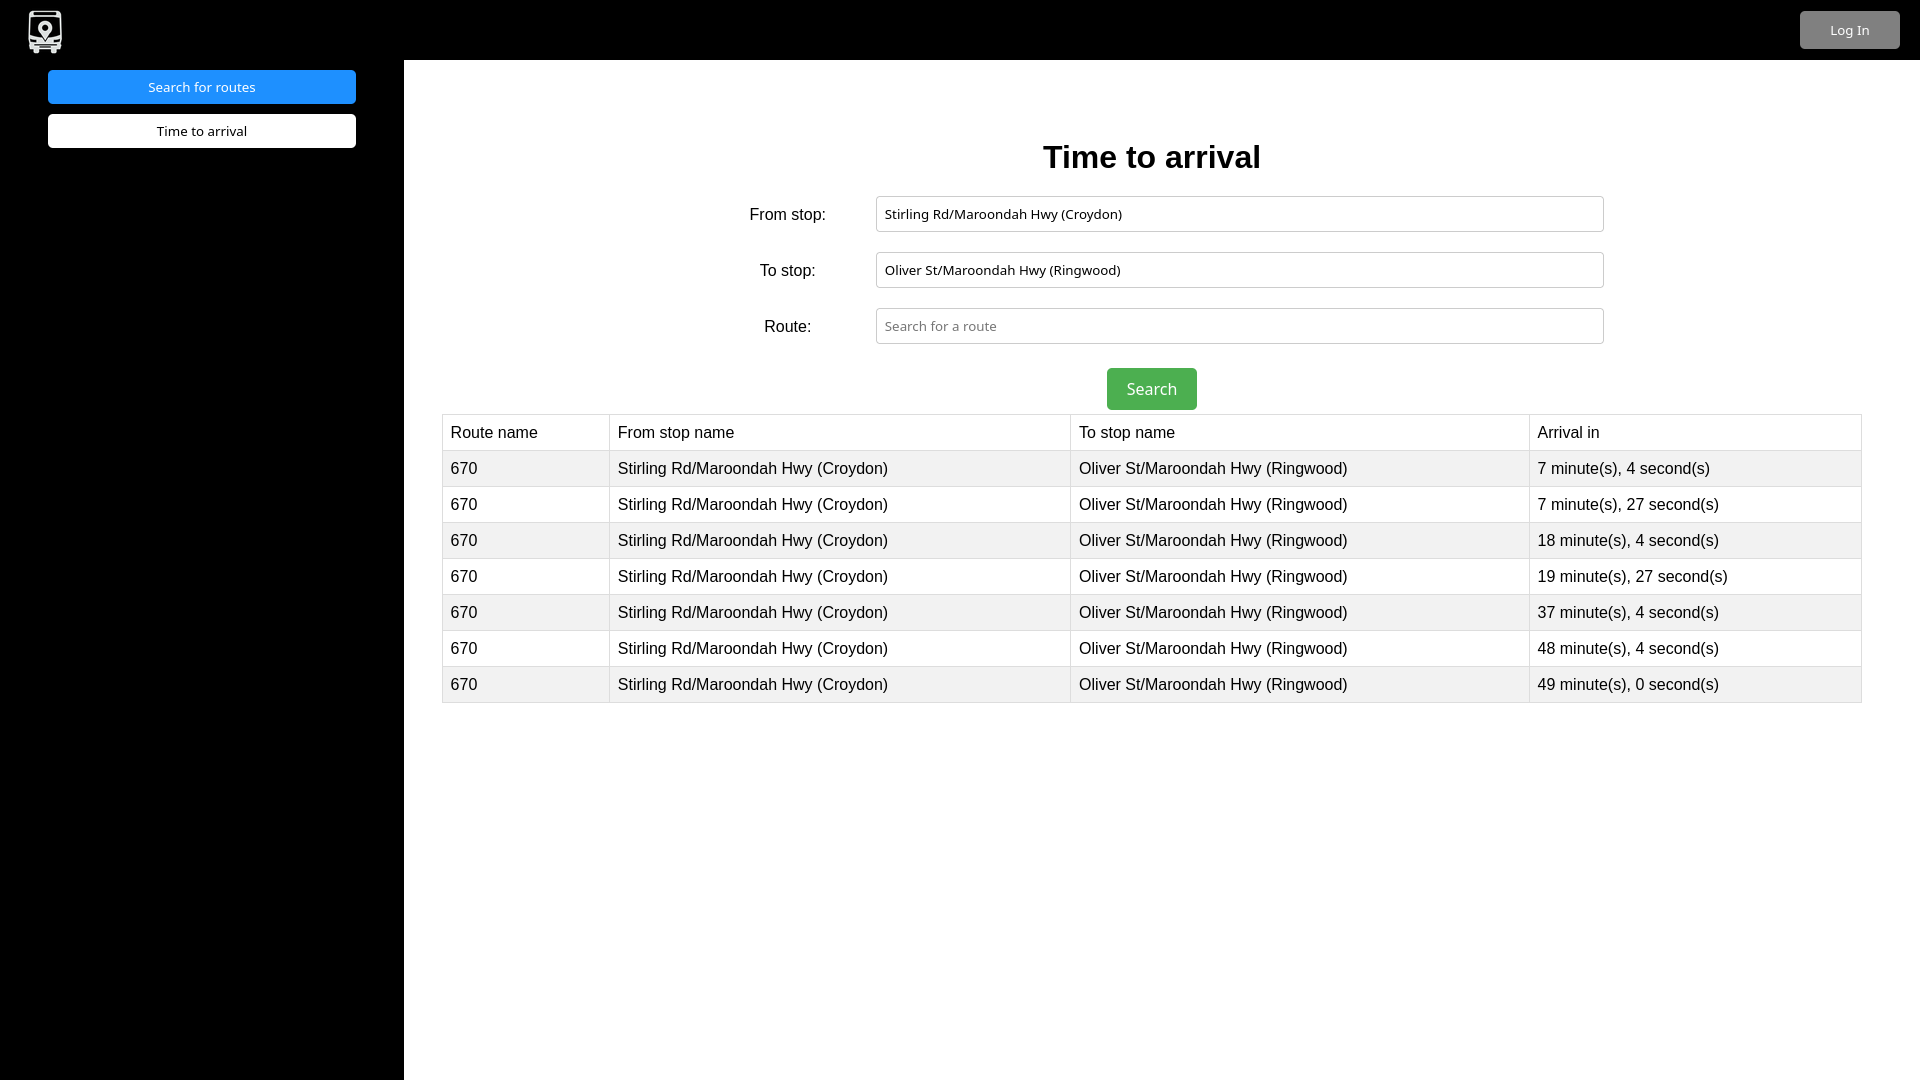
\includegraphics[scale=0.3]{3}
\caption{Отримання часу прибуття транспортного засобу на вказану зупинку на вказаному маршруті.}
\end{figure}

\begin{figure}[H]
	\centering
	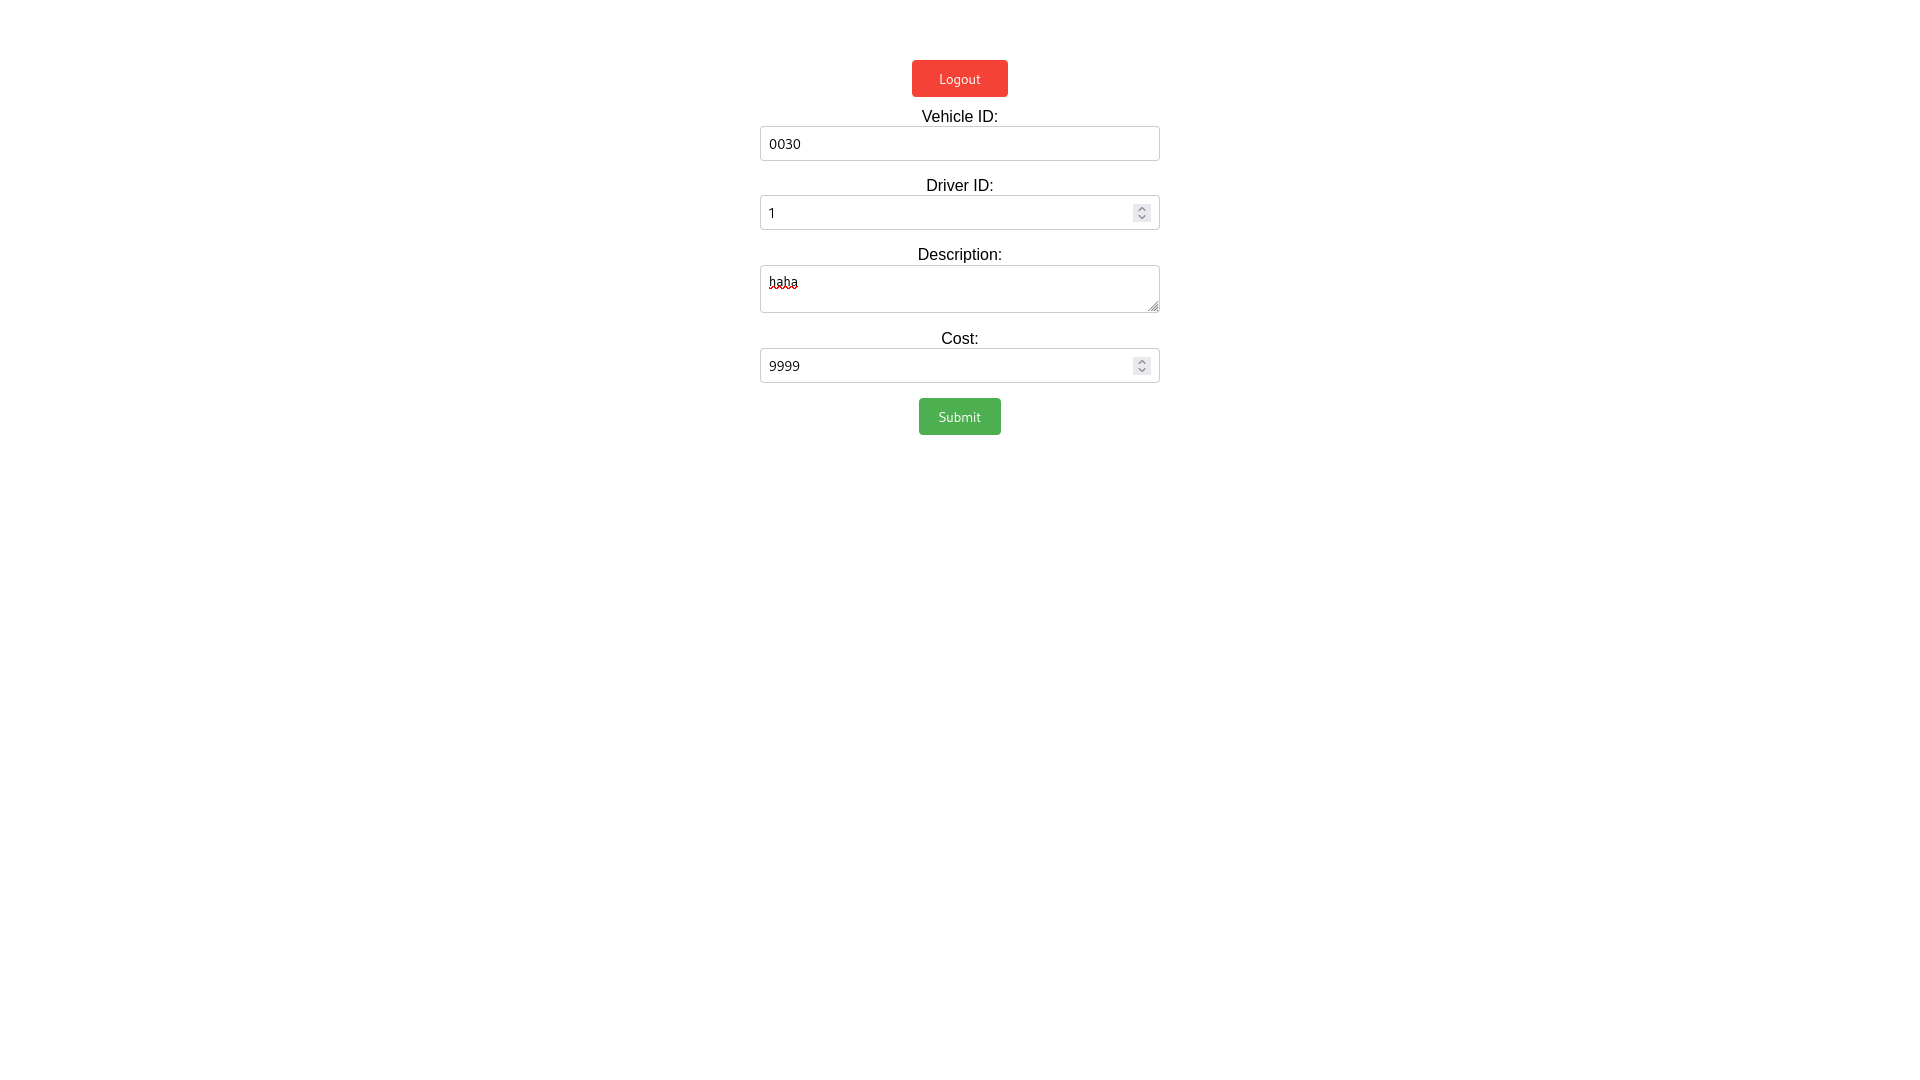
\includegraphics[scale=0.3]{4}
	\caption{Сторінка авторизації.}
\end{figure}

Користувачі, авторизовані з роллю \textit{driver}, мають можливість внести запис про технічне обслуговування, та отримати деталі маршруту.

\begin{figure}[H]
\centering
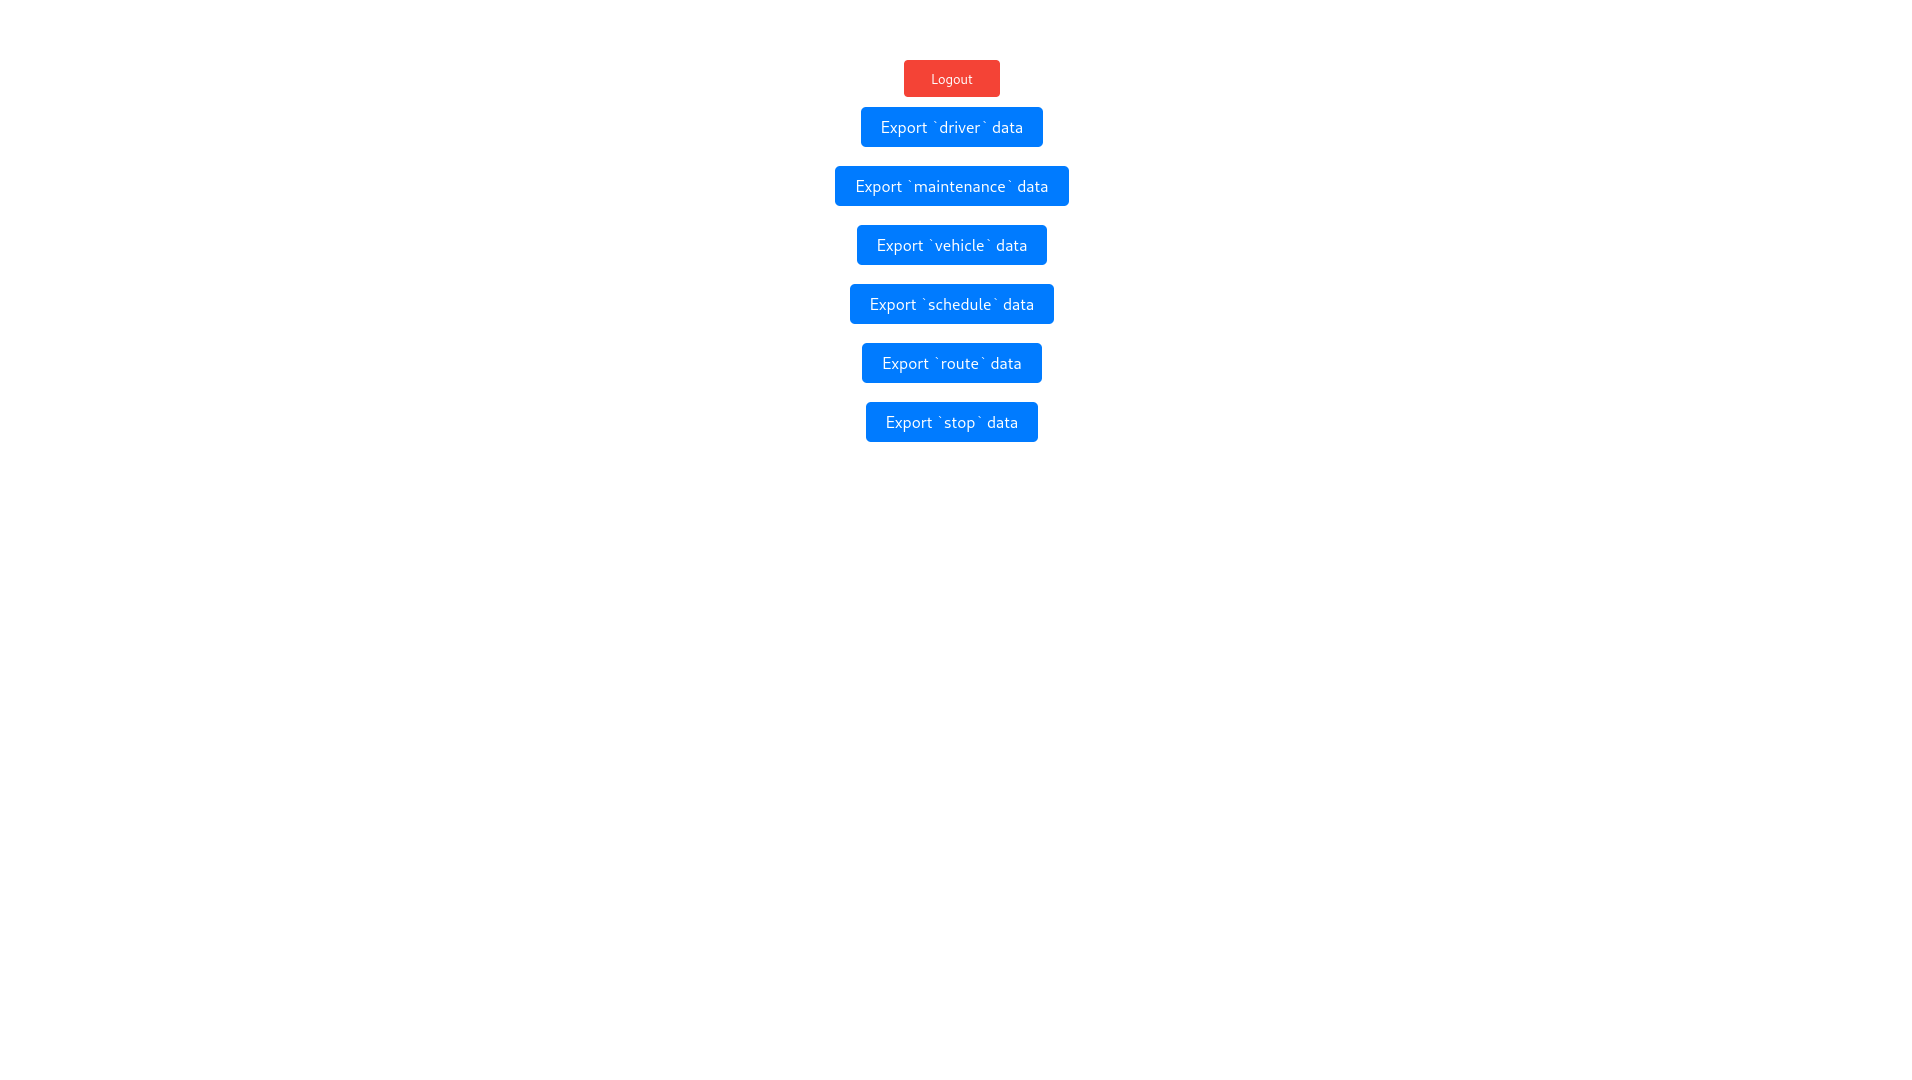
\includegraphics[scale=0.25]{5}
\caption{Внесення запису про технічне обслуговування транспортного засобу.}
\end{figure}

Користувачі, авторизовані з роллю \textit{manager}, мають можливість експортувати дані у форматі \textit{JSON}, та переглядати статистику та дані у базі даних.

\begin{figure}[H]
\centering
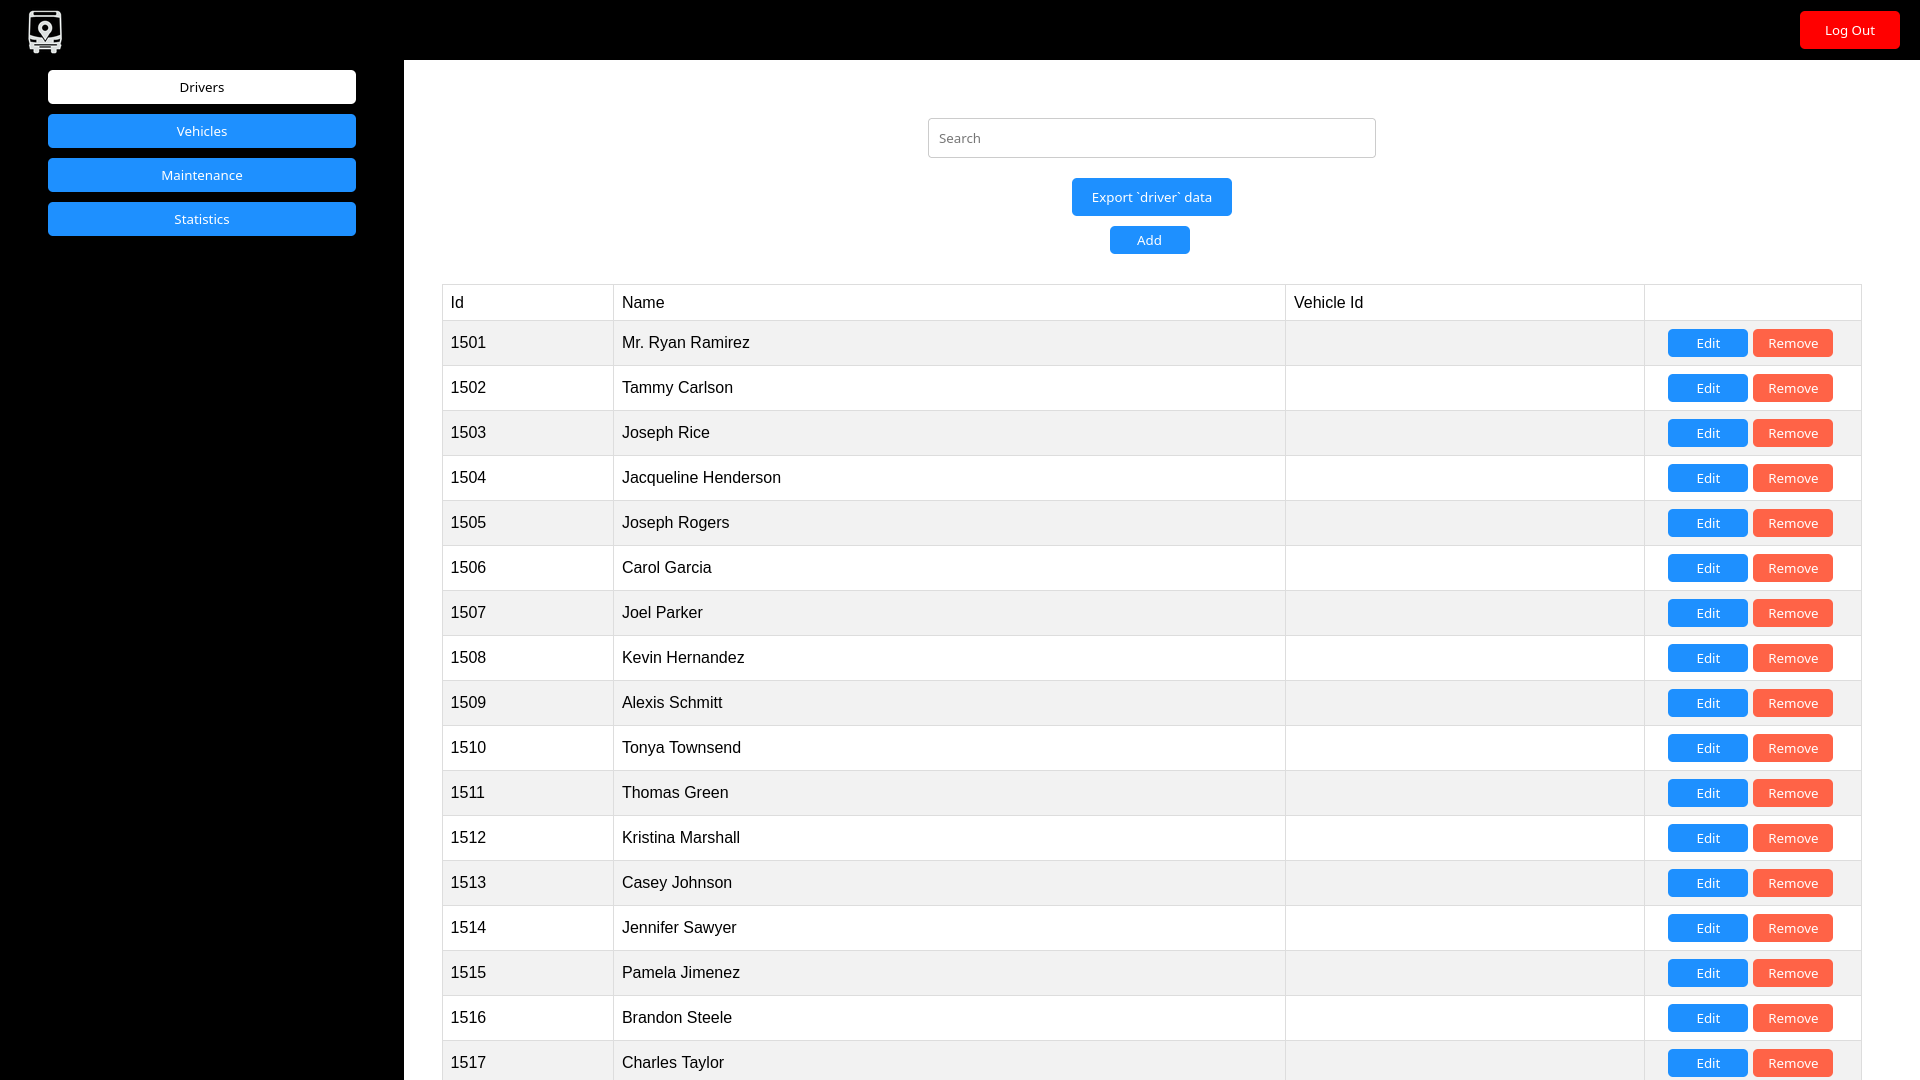
\includegraphics[scale=0.3]{6}
\caption{Вигляд засобу відображення даних про водіїв.}
\end{figure}

\begin{figure}[H]
	\centering
	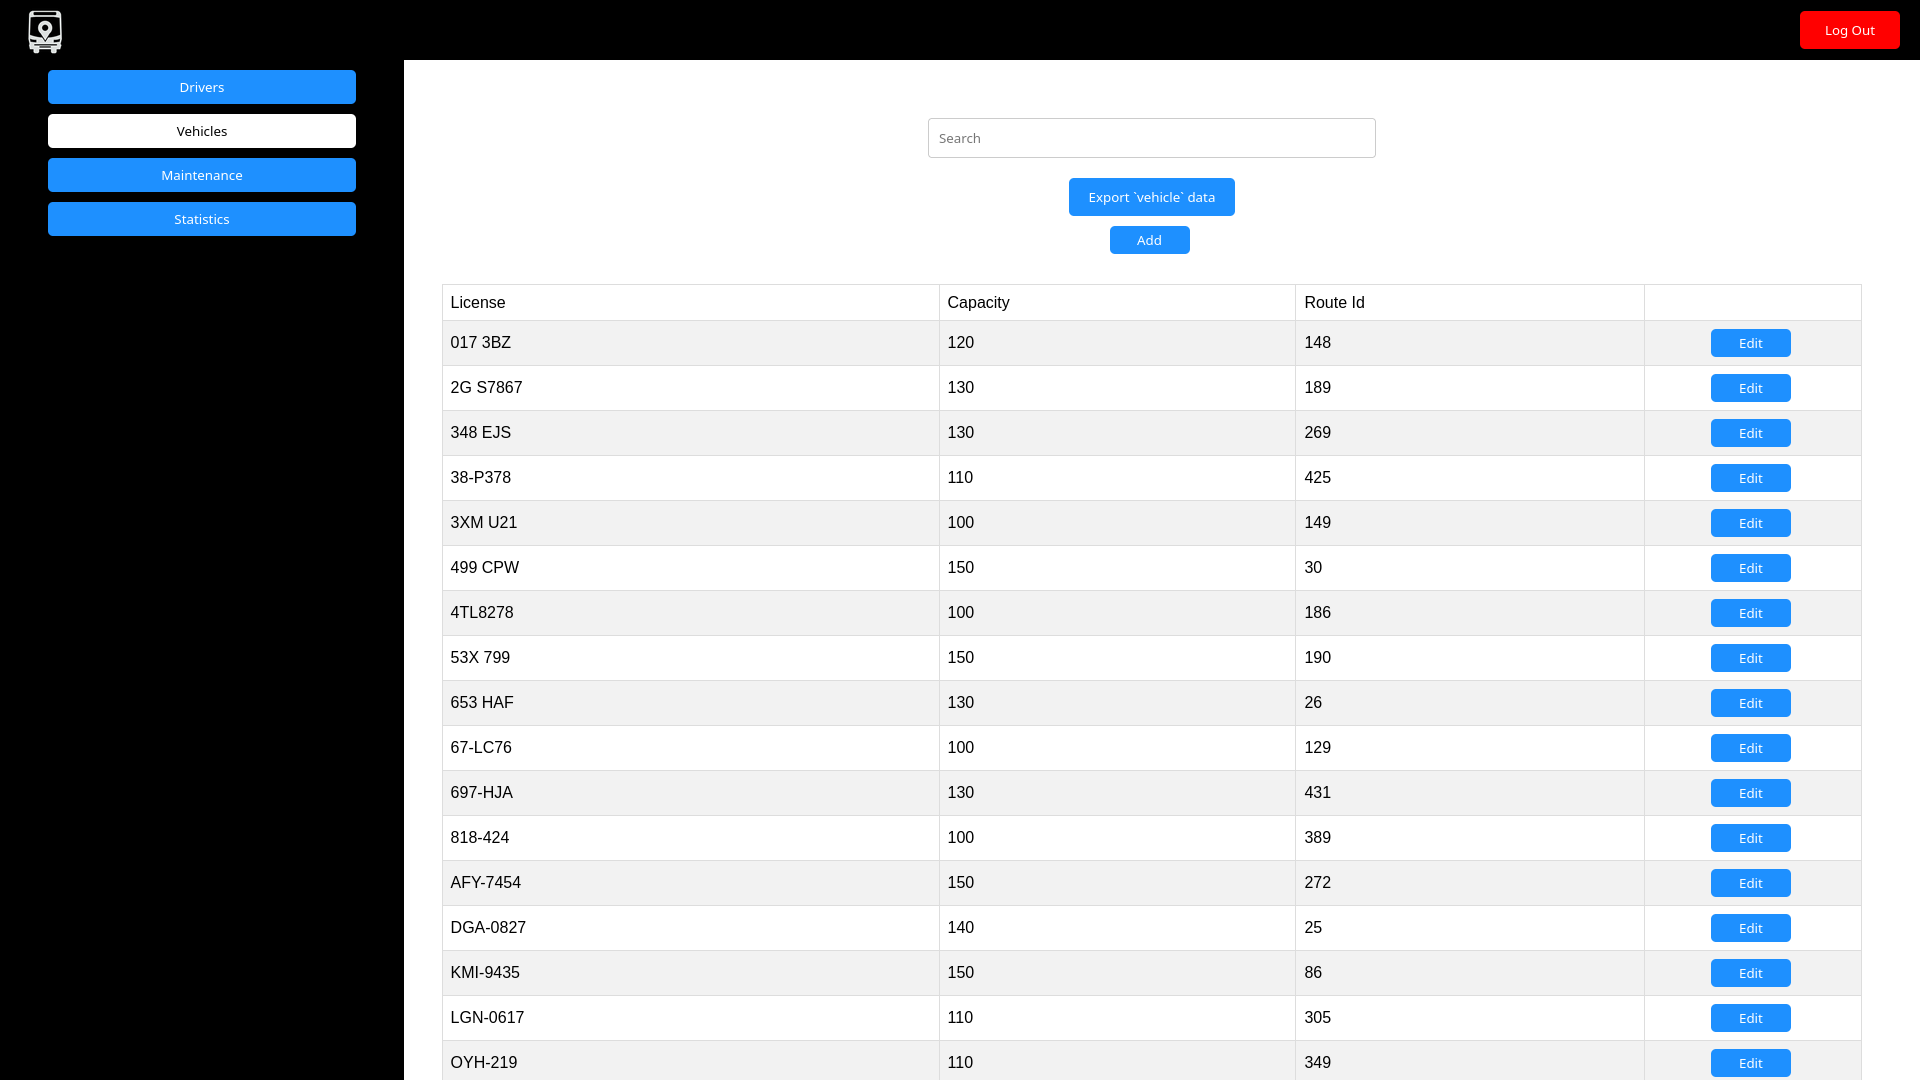
\includegraphics[scale=0.3]{7}
	\caption{Вигляд засобу відображення даних про транспортні засоби.}
\end{figure}

\begin{figure}[H]
	\centering
	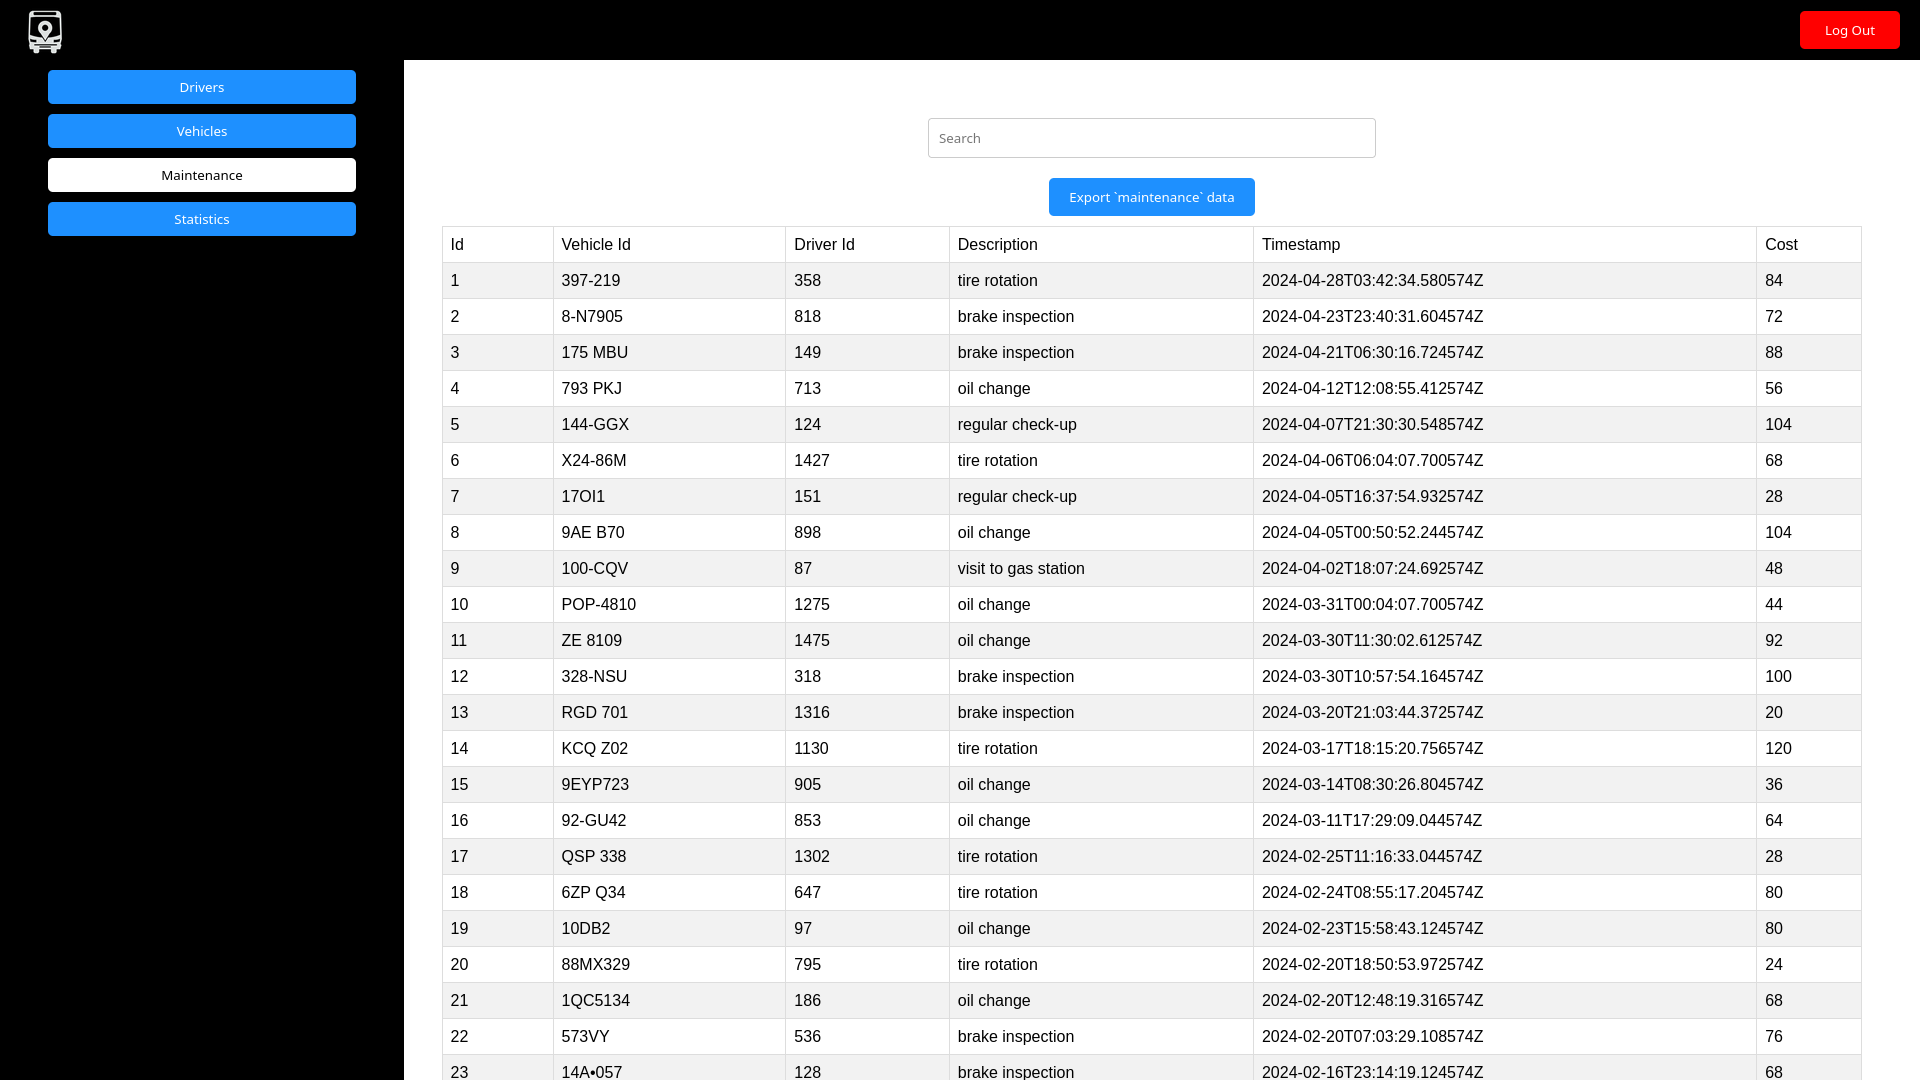
\includegraphics[scale=0.3]{8}
	\caption{Вигляд засобу відображення даних про технічне обслуговування.}
\end{figure}

\subsection{Засоби аналітичного представлення даних}

\begin{figure}[H]
	\centering
	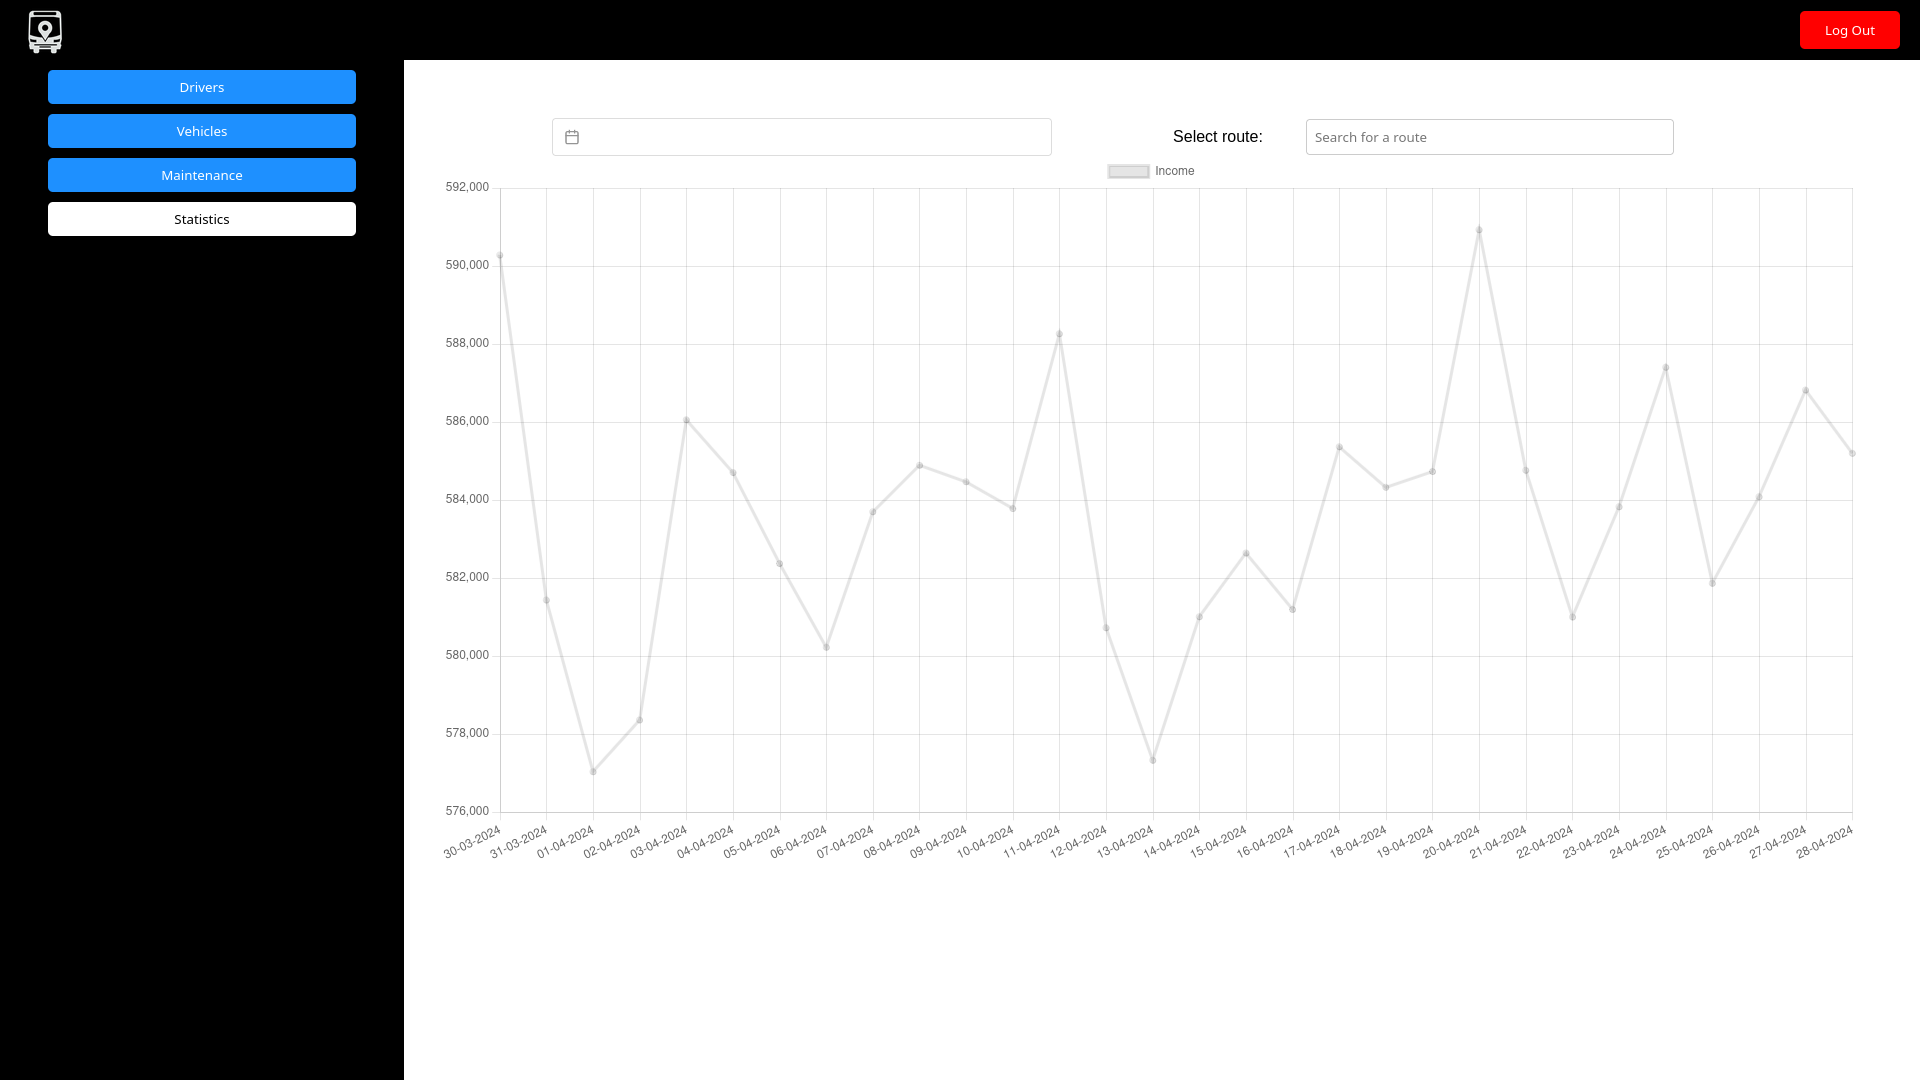
\includegraphics[scale=0.3]{10}
	\caption{Вигляд засобу аналітичного представлення даних.}
\end{figure}

\subsection{Засоби експорту даних}
% Обмеження
Програмна система дозволяє експорт будь-яких таблиць лише в одному форматі, що може становити обмеження у випадках, коли інші формати бажані для взаємодії з різноманітними інструментами або системами.

% Формат файлу
Програмна система дозволяє експортувати дані вказаної таблиці, у такому вигляді, як вони зберігаються у базі даних, у форматі \textit{JSON}. Цей формат забезпечує зручність у взаємодії з іншими програмами та забезпечує можливість збереження ієрархічної структури даних. Крім того, \textit{JSON} є легким для розуміння і обробки як людьми, так і комп'ютерами, що робить його ідеальним вибором для експорту даних.

\subsection{Засоби програмного інтерфейсу}
Програмний інтерфейс системи дозволяє виконувати наступні дії за допомогою \textit{HTTP} запитів:
\begin{itemize}
\item Шукати зупинки за назвою.
\item Шукати маршрути за назвою.
\item Шукати маршрути. що містять вказані зупинки.
\item Отримувати час прибуття транспортного засобу на вказаній зупинці та на вказаному маршруті.
\item Створювати транзакцію.
\item Отримувати наступну зупинку після вказаної на вказаному маршруті.
\item Експортувати дані вказаних таблиць у форматі JSON.

\end{itemize}

\newpage

\section*{Висновки}
\setcounter{subsection}{0}
\addcontentsline{toc}{section}{Висновки}
\subsection{Встановлені недоліки}
Під час створення інформаційної системи для компанії з регулярних перевезень було виявлено наступні недоліки:
\begin{itemize}
\item Запити до програмного інтерфейсу, які повертають увесь вміст бази даних, можуть призвести до низької продуктивності системи. Це може бути особливо важливо при роботі з великими обсягами даних.
\item Інтерфейс користувача системи потребує покращення для забезпечення зручності та ефективності взаємодії з системою. Важливо забезпечити інтуїтивно зрозумілий та привабливий для користувача інтерфейс.
\end{itemize}

\subsection{Перспективи покращення}
Для подолання встановлених недоліків можна реалізувати наступне:
\begin{itemize}
\item Для спрощення обліку транзакцій можна реалізувати інтеграцію з банківською системою. Це дозволить автоматизувати процеси оплати та обліку коштів пасажирів.
\item Необхідно провести аналіз та оптимізацію запитів до бази даних, щоб зменшити навантаження на систему та покращити її продуктивність.
\item Розробка мобільного додатка для пасажирів дозволить забезпечити зручний доступ до інформації про розклад руху та покупку квитків. Окрема система для адміністраторів та водіїв дозволить керувати функціями та даними, що відповідають їхнім потребам та відповідальностям.
\end{itemize}

\newpage

\section*{Список літератури}
\setcounter{subsection}{0}
\addcontentsline{toc}{section}{Список літератури}

\begin{enumerate}
\item Джерело первинних історичних даних (Електронний ресурс). \\Посилання: \href{https://www.researchgate.net/publication/325161554_A_collection_of_public_transport_network_data_sets_for_25_cities}{https://www.researchgate.net/publication/325161554-A-collection-of-public-transport-network-data-sets-for-25-cities}
\item Документація Golang (Електронний ресурс). \\Посилання: \href{https://go.dev/doc/}{https://go.dev/doc/}
\item Документація Vue.js (Електронний ресурс). \\Посилання: \href{https://vuejs.org/guide/introduction.html}{https://vuejs.org/guide/introduction.html}
\item Документація PostgreSQL (Електронний ресурс). \\Посилання: \href{https://www.postgresql.org/docs/}{https://www.postgresql.org/docs/}
\end{enumerate}

\newpage

\section*{Додатки}
\setcounter{subsection}{0}
\addcontentsline{toc}{section}{Додатки}
\subsection{Скрипт створення бази даних та завантаження історичних даних}
{\fontsize{8pt}{8pt}\selectfont\lstinputlisting{import.sh}}

\subsection{Інший програмний код}
Файл \textit{main.go}
{\fontsize{8pt}{8pt}\selectfont\lstinputlisting{src/main.go}}

Файл \textit{models.go}
{\fontsize{8pt}{8pt}\selectfont\lstinputlisting{src/models/models.go}}

Файл \textit{App.Vue}
{\fontsize{8pt}{8pt}\selectfont\lstinputlisting{src/f/src/App.vue}}

\end{document}
